\section{Evaluation}
\label{sec:evaluation}

In this section, we report on the results of an extensive experimental
evaluation of our approach.  We fully implemented \VMS\ in Java and
integrated it with Apache \HB. Before we discuss our results, we
review the experimental set-up and the workload.

%\subsection{Experimental set-up}  

%
% aj - below, the numbers do not add up, please fix/clarify
%             I removed reference to machines, as we say nodes
%
%\subsection{Experimental set-up} 
\noindent
{\bf Experimental set-up} --
 All experiments were performed on a cluster comprised of 40 nodes
(running Ubuntu 14.04). Out of these, 11 were dedicated to the Apache
Hadoop (v1.2.1) installation, one as name node (HDFS master) and 10 as
data nodes (HDFS file system). On HDFS, we installed \HB\ (v0.98.6.1)
with one master and 10 region servers. On every region server, we
deployed one of our extensions (cf. Figure~\ref{fig:kv_model}). View
managers (\VMs) were deployed on 20 separate nodes to be able to scale
without interfering with the core system (i.e., the 12 \HB\ nodes.)
Finally, another 8 nodes were reserved for \HB\ clients to generate
the update load on base tables.

Prior to each experiment, we created an empty base table and defined a
set of view tables. View definitions and underlying base tables are
maintained as meta data in a separate \textit{view definition}
table. By default, \HB\ stores all base table records in one
region. We configured \HB\ to split every table into 50 parts. This
choice allows \HB\ to balance regions with high granularity and
ensures a uniform distribution of keys among available region servers.

\begin{figure*}
\minipage{0.32\textwidth}
  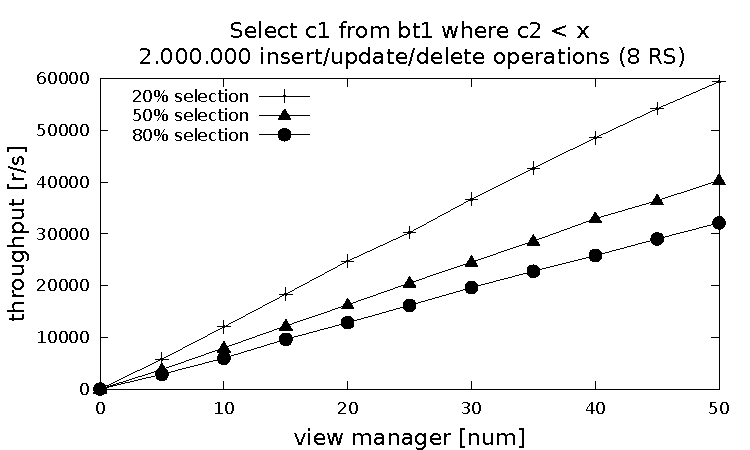
\includegraphics[width=\linewidth]{figures/selection}
      \vspace{-3mm}
  \caption{Selection performance}\label{fig:selection}
        \vspace{-1mm}
\endminipage\hfill
\minipage{0.32\textwidth}
  \includegraphics[width=\linewidth]{figures/aggregation}
      \vspace{-3mm}
  \caption{Aggregation performance}\label{fig:viewtypes}
        \vspace{-1mm}
\endminipage\hfill
\minipage{0.32\textwidth}%
  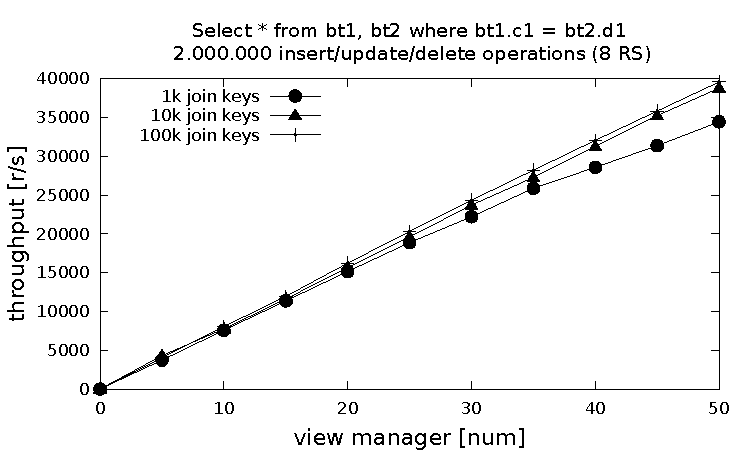
\includegraphics[width=\linewidth]{figures/join}
      \vspace{-3mm}
  \caption{Join performance}\label{fig:join}
        \vspace{-1mm}
\endminipage
\end{figure*}

For \texttt{COUNT}, \texttt{SUM}, \texttt{MIN}, and \texttt{MAX}
views, we created base tables that contain one column $c_1$
(aggregation key) and another column $c_2$ (aggregation value).  We
choose a random number $r_a$ between $1$ and some upper bound $U$ to
generate aggregation keys.  We can control the number of base table
records that affect one particular view table record. For the
\texttt{SELECTION} view, we use the same base table layout and apply
the selection condition to column $c_2$. The \texttt{JOIN} view
requires two base tables with different row keys. The row key of the
right table is stored in a column in the left table, referred to as
foreign key.

The workload we generate consists of \textit{insert}, \textit{update}
and \textit{delete} operations that are issued to HBase using its
client API. Operations are generated according to different
distributions over the key space (we use Zipf and Uniform).  A Zipf
distribution simulates a ``hot data'' scenario, where only few base
table records are updated very frequently.


%\subsection{Experiments} 

With our experiments, we primarily evaluate the performance of the
system with regards to throughput and view maintenance latency.

\noindent
{\bf Impact of view type on throughput} -- First, we evaluate the
performance for every view type, separately. We measure the throughput
during view maintenance, i.e., the number of updates a view can
sustain per second.  We configure a system with a fixed number of 10
region servers to host all tables. The number of \VMs\ varies between 10
to 50, and all \VMs\ are assigned evenly to region servers. Furthermore,
40 clients generate a total of 1 million operations per
experiment. Updates are concurrently processed by all \VMs. The
experiments are completed after all clients sent their updates and all
\VMs\ emptied their queues.

For the \texttt{SELECTION} view, we experimented with three different
selectivity levels (i.e., selection of 10, 50 and 90 percent of base
records), while varying the number of \VMs\ that process the update
load. Figure~\ref{fig:selection} shows the results.  The
\texttt{SELECTION} view is not realized with an auxiliary
view. Compared to the other views, its maintenance results in the
highest throughput.  The performance depends on the amount of records
selected. Interesting is that the absolute throughput is limited by
the throughput clients exert on the system. In
Figure~\ref{fig:selection}, the performance is monotonically
decreasing for a selectivity of 10\%. This means, \VMs\ propagate
updates as fast as they are applied to \HB\ by clients. Increasing
the number of \VMs\ only slows down the system as more components are
running concurrently.

Figure~\ref{fig:viewtypes} shows the performance of the aggregation
view types: \texttt{COUNT}, \texttt{SUM}, \texttt{MIN}, \texttt{MAX},
and \texttt{INDEX}. Again, we use a fixed configuration comprised of
10 region servers and 40 clients that generated 1M operations.
Aggregation views derive from an auxiliary view (here a \texttt{DELTA}
view.)  Therefore, the throughput for aggregation views is lower than
for the \texttt{SELECTION} view. However, in contrast to the
\texttt{SELECTION} view, the throughput significantly benefits from
increasing the number of \VMs. Not surprisingly, \texttt{COUNT} and
\texttt{SUM} views show similar performance, as their maintenance is
nearly identical.  \texttt{INDEX} view maintenance exhibits a lower
throughput than \texttt{COUNT} and \texttt{SUM}, which only store one
attribute for the aggregated value, whereas the \texttt{INDEX} view
stores a variable number of primary keys associated with the index
column value of the indexed table.  The performance of both
\texttt{MIN} and \texttt{MAX} is worse compared to the \texttt{INDEX}
view. In a \texttt{MIN} (max) view, we also store base table records,
together with the aggregated value.  The storage overhead is equal to
\texttt{INDEX}, but sometimes the values of an entire row needs to be
queried to recalculate the new minimum (maximum).  


Figure~\ref{fig:join} shows the results for the \texttt{JOIN} view
under the same conditions as above. Compared to the other view types
and not surprising, \texttt{JOIN} shows lower throughput.  The
\texttt{JOIN} view requires a more complex internal auxiliary view
table constellation and maintenance. However, we suspect that
throughput is still higher than as if full table scans would have to
be used to find matching rows (not considering consistency issues, if
scans would be used.)  Similar to aggregation views, \texttt{JOIN}
benefits from an increased number of view managers. Also, here as
well, auxiliary tables for \texttt{JOIN} can be amortized as more
views are defined.

%\begin{figure*}
%\minipage{0.32\textwidth}
%  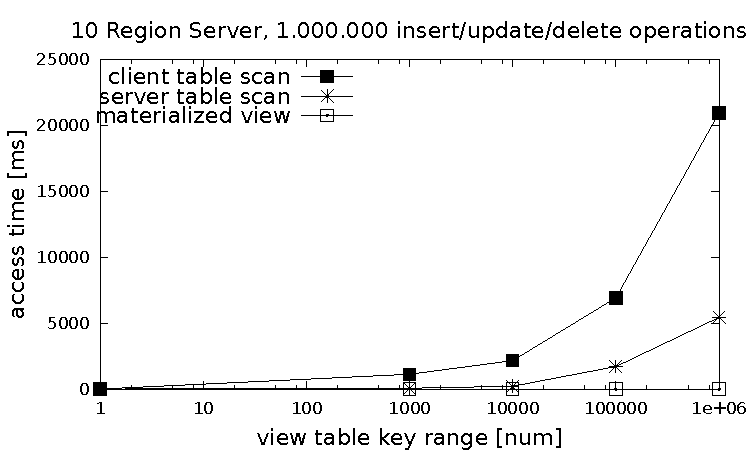
\includegraphics[width=\linewidth]{figures/benefit}
%      \vspace{-3mm}
%  \caption{Benefit of view maintenance}\label{fig:benefits}
%        \vspace{-1mm}
%\endminipage\hfill
%\minipage{0.32\textwidth}
%  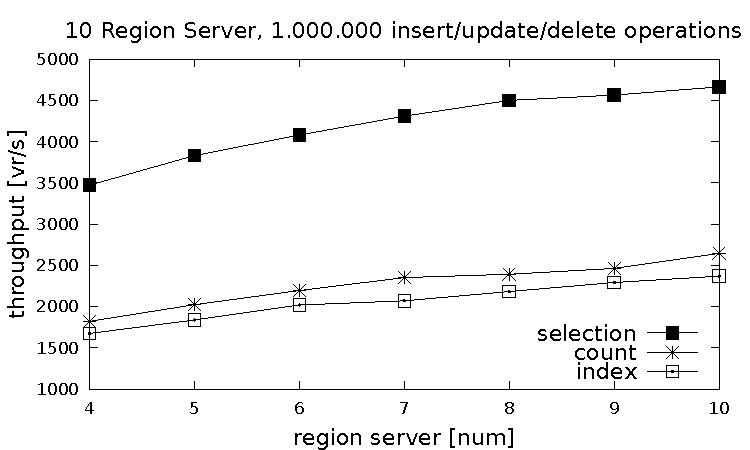
\includegraphics[width=\linewidth]{figures/scale_rs}
%      \vspace{-3mm}
%  \caption{Scale region servers}\label{fig:regionservers}
%        \vspace{-1mm}
%\endminipage\hfill
%\minipage{0.32\textwidth}%
%  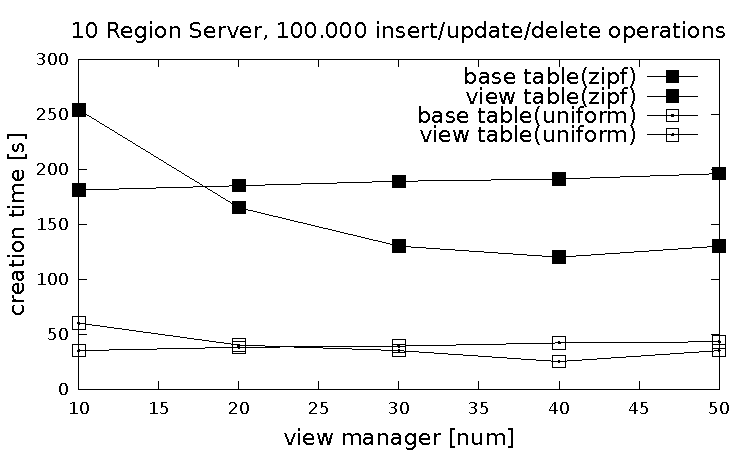
\includegraphics[width=\linewidth]{figures/zipf}
%      \vspace{-3mm}
%  \caption{Zipf distribution}\label{fig:zipf}
%        \vspace{-1mm}
%\endminipage
%\end{figure*}
%\begin{figure*}
%\minipage{0.32\textwidth}
%  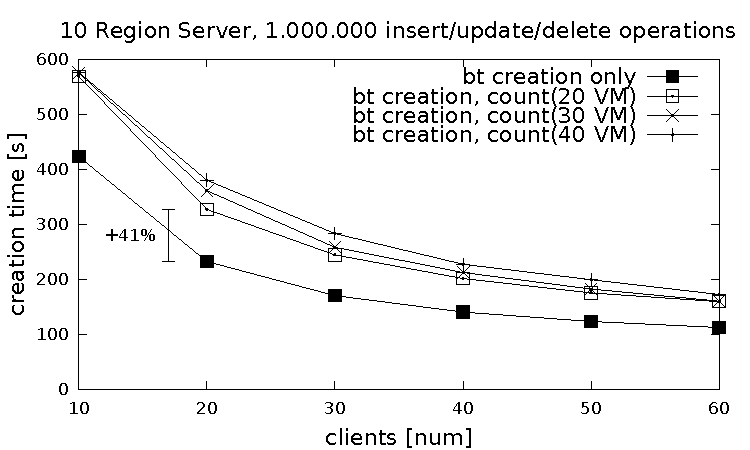
\includegraphics[width=\linewidth]{figures/cost}
%      \vspace{-3mm}
%  \caption{Cost of view maintenance}\label{fig:cost}
%      \vspace{-1mm}
%\endminipage\hfill
%\minipage{0.32\textwidth}
%  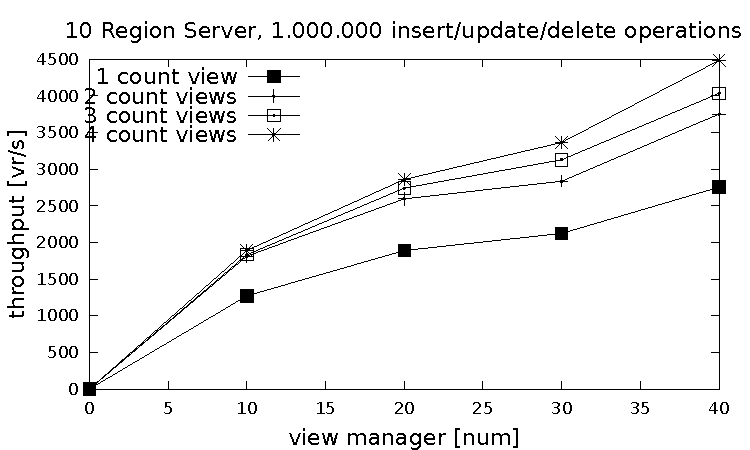
\includegraphics[width=\linewidth]{figures/scale_views}
%      \vspace{-3mm}
%  \caption{Scale views}\label{fig:views}
%      \vspace{-1mm}
%\endminipage\hfill
%\minipage{0.32\textwidth}%
%  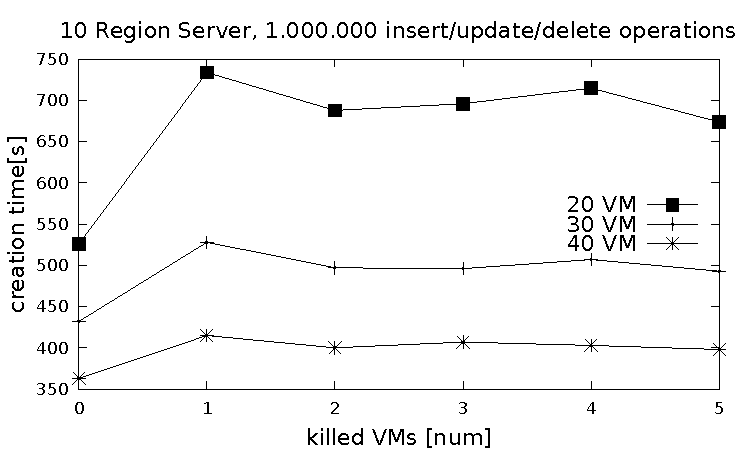
\includegraphics[width=\linewidth]{figures/killvm}
%      \vspace{-3mm}
%  \caption{Fault tolerance}\label{fig:killvm}
%      \vspace{-1mm}
%\endminipage
%\end{figure*}

%\begin{tikzpicture}
%\begin{axis}[
%ybar,
%enlargelimits=0.15,
%legend style={at={(0.5,-0.15)},
%anchor=north,legend columns=-1},
%ylabel={\#participants},
%symbolic x coords={select,aggregation,join},
%xtick=data,
%nodes near coords,
%nodes near coords align={vertical},
%]
%\addplot coordinates {(select,810) (aggregation,9) (join,4)};
%\addplot coordinates {(select,1280) (aggregation,4) (join,4)};
%\addplot coordinates {(select,1670) (aggregation,1) (join,1)};
%\legend{used,understood,not understood}
%\end{axis}
%\end{tikzpicture}




\noindent
{\bf Cost and benefit of view maintenance} -- To determine the
benefits, i.e., the latency improvement a client experiences when
accessing a view, and the costs, i.e., essentially, the decrease in
overall system throughput that results, we conducted an experiment
with three different view maintenance strategies: (i) \textit{Client
  table scan}: To obtain the most recent count view values, a client
scans the base table and aggregates all values on its own. (ii)
\textit{Server table scan}: To obtain the most recent count view
values, the client sends a request to \HB, which internally computes
the view in a custom manner and returns it as output. In the
implementation, we use \HB's ability to parallelise table access.  All
region servers scan their part of the table and, at the end,
intermediate results are collected and merged.  (iii)
\textit{Materialized view}: Views are maintain incrementally by
\VMS\ configured with 40 \VMs\ used to materialize the count view in
parallel.  For (i) and (ii), we disregard inconsistencies that may
result from concurrent table updates while scans are in progress
(certainly noting that in practice, this would not be an option; thus,
these two approaches are merely serving as a baseline, here.) Our
primary objective is to obtain some feel for how \VMS\ fares relative
to other potential approaches.

The results are given in Figure~\ref{fig:benefits}, where we measure
the latency a client perceives (i.e., the time until results are
available) as the scanned key range increases.  The first strategy
performed worst. \textit{Client table scans} are sequential by nature
and require a large number of RPCs to \HB, even if requests are
batched. Especially, with increasing table size, this approach becomes
more and more impracticable.



\textit{Server table scan} is promising because \HB\ is able to
exploit the data distribution, which results in a linear speed-up.
Nonetheless, the time to obtain the most recent values for a count
aggregate reached 5~s for a table with 1M rows.  While this result
could now be cached in materialized form, in scenarios with frequently
changing base data, recalculations would have to be frequently
repeated to keep the results up-to-date. Moreover, concurrent table
scans may interfere with the write performance of region servers.

Because views are materialized and updates are done incrementally,
latencies for the third strategy are exactly the same as for every
\HB\ table. Moreover, the client only accesses the aggregated values
and not the base table. Therefore, the latency remains below 1~ms,
even for a base table with 10 million rows.

Materializing views come at a cost. We assess this cost as the
performance impact on base table creation time (here, defined as the
time to insert 1M tuples into the base table.)  Figure~\ref{fig:cost}
shows the base table creation time with and without concurrent view
maintenance.  We track creation time as the number of clients
increases.  Figure~\ref{fig:cost} shows view maintenance with 20, 30
and 40 \VMs.  While view maintenance increases the base table creation
time by approximately 40\%, a further increase of \VMs\ (by ten) only
increases base table creation time by approximately 2\%.

\noindent
{\bf System scalability} -- Figure~\ref{fig:selection} and
Figure~\ref{fig:viewtypes} show the performance of different view
types. In both experiments, we increased the number of \VMs.  Now, we
examine system performance when scaling up region servers. In
Figure~\ref{fig:regionservers}, the number of region servers is varied
from 4 to 10. We run the experiment with a selection, a count and an
index view and measure throughput. We observe an almost linear
increase of throughput independent of the view type processed.

The effect can be explained as follows: Each region server runs on a
separate node. Adding another region server results in additional I/O
channels (i.e., separate disk).  Thus, the overall performance of
\HB\ increases. Client requests are completed faster due to the
additional I/O capacity.  Likewise, \VMs\ can perform faster view
updates.  We draw the following conclusion: Scaling up the number of
\VMs\ as in Figure~\ref{fig:selection} and Figure~\ref{fig:viewtypes}
improves the view maintenance throughput up to a point where \VMs\ are
saturated with updates that they can push through the available I/O
channels.  Scaling up the region server improves overall performance,
also for \VMs, due to the additional I/O capacity.

Figure~\ref{fig:views} shows system throughput as multiple views are
maintained by a varying number of \VMs.  We note a performance leap as
load changes from maintaining one to two count views. In our workload
the count views derive from the same auxiliary table, which must be
maintained as well, but only once. In further increasing the number of
views, the effect diminishes.  All aggregation views, especially join
views, benefit from the sharing of auxiliary views.

However, increasing the number of views in the system, also increases
the lag between base table states and derived view table states. While
our view states always remain consistent, they do lag behind in time.
This lag can be reduced by increasing the number of \VMs\ to speed up
view maintenance.  Thus, the more views we maintain, the more
important is the number of \VMs\ allocated.

\begin{figure}
  \includegraphics[width=\linewidth]{figures/bar}
      \vspace{-3mm}
  \caption{Selection performance}\label{fig:staleness}
        \vspace{-1mm}
\end{figure}

\noindent
{\bf Impact of data distribution} -- Figure~\ref{fig:zipf} evaluates
the effect of different distributions on system performance.  We scale
the number of \VMs\ and track the latency for creating base tables and
derived views.  Keys of update operations are drawn from a Zipf and a
Uniform distribution.

For the Uniform distribution, creation latencies are independent of
the number of \VMs\ assigned, even a small number of \VMs\ can handle the
load in our set-up.  For the Zipf distribution, latencies are much
higher. We also see that creation and maintenance latency increase,
yet, are positively effected by increasing the number of \VMs\ that
propagate updates.  Thus, especially for a skewed workload, the system
greatly benefits from being able to dynamically assign \VMs.  \VMs\ can
be assigned to hot spots in the key range, away from ranges where they
are not needed.  Nevertheless, in this case, \HB\ may constitute a
bottleneck for clients. Clients issue updates to a set number of
region servers that handle 90\% of the load, thus, resulting in a
slowdown.  \HB\ developers suggest that keys of updates should be
salted. That is a prefix is assigned to keys, such that their
distribution becomes uniform again. In this case, \VMs\ propagate
updates as we saw above.

\noindent
{\bf Impact of VM crash} -- Figure~\ref{fig:killvm} shows the impact
of a view manager crash on system performance.  In this experiment, we
track view maintenance latency, as the number of \VMs\ available in the
system crashes.  We ran experiments with 20, 30 and 40 \VMs,
respectively. Twenty seconds after view maintenance started, we
terminate a number of \VMs. In this experiment, the \VMs\ are distributed
evenly to region servers. In a set-up with 20 \VMs\ and 10 region
servers, we have a ratio of 2 \VMs\ per region server. Terminating both
\VMs\ of the same region server stops view maintenance. The operations
arriving at that region server cannot be forwarded until a new \VM\ is
assigned to the region server. In the experiment, we terminate \VMs\ of
different region servers.

In our set-up, a single crashing \VM\ reduces the view maintenance
latency, because it takes additional time for recovery to replay the
transaction log and because the remaining \VMs\ have to absorb
additional load.  The failing of further \VMs\ does not further impact
the situation.  As long as every region server loses only one of its
two \VMs, the overall processing time remains the same.  Overall, the
impact of a \VM\ crash lessens, the more \VMs\ are deployed.  Thus,
increasing the number of \VMs, increases the fault resilience of the
system.

